\documentclass[10pt,aspectratio=169,dvipsnames]{beamer}
\usetheme[]{Berlin}

\setbeamertemplate{footline}{
  \usebeamercolor[fg]{framesource}%
  \usebeamerfont{page number in head}%
  \hspace{0.2cm}
  \small \insertframenumber
  \vspace{0.2cm}
  % \doclicenseIcon
  % \hfill
  % \includegraphics[height=0.8cm]{graphics/tublogo.pdf}
  % \hspace{0.2cm}
}

\setbeamercovered{transparent}

\setbeamertemplate{footline}[
 myframe number]

% PACKAGES
\usepackage[absolute,overlay]{textpos}
\usepackage[utf8]{inputenc}
\usepackage[official]{eurosym}
\usepackage{booktabs}
\usepackage{parskip}
\usepackage{bm}
\usepackage{tikz}
\usepackage{adjustbox}
\usepackage{hyperref}
\usepackage{qrcode}

\usepackage[
    type={CC},
    modifier={by},
    version={4.0},
]{doclicense}

% HYPERREFERENCES
\usepackage{hyperref}
\hypersetup{
	colorlinks=true,
	citecolor=tub-blue,
	linkcolor=tub-blue,
	urlcolor=tub-blue
}

\usepackage[sfdefault]{roboto}
\usepackage[normalem]{ulem}
\usepackage{multicol}

% GRAPHICS
\graphicspath{
  {../../papers/import-benefits/slides/graphics/},
  {graphics/}}
\DeclareGraphicsExtensions{.pdf,.jpeg,.png,.jpg}

% FORMATTING
\setlength{\parskip}{6pt}
\linespread{1.1}
\newcommand{\seprule}{\par\noindent\textcolor{black!25}{\rule{\textwidth}{0.4pt}}}

% SOURCES
\setbeamercolor{framesource}{fg=gray}
\setbeamerfont{framesource}{size=\tiny}
\newcommand{\source}[1]{\begin{textblock*}{5cm}(8.6cm,8.25cm)
    \begin{beamercolorbox}[ht=0.5cm,right]{framesource}
        \usebeamerfont{framesource}\usebeamercolor[fg]{framesource} Source: {#1}
    \end{beamercolorbox}
\end{textblock*}}

% COLOR TEXT
\newcommand{\bl}[1]{\textcolor{tub-blue}{#1}}
\newcommand{\gr}[1]{\textcolor{tub-green}{#1}}
\newcommand{\rd}[1]{\textcolor{tub-red}{#1}}
\newcommand{\yl}[1]{\textcolor{tub-yellow}{#1}}
\newcommand{\cb}[1]{\colorbox{gray!20}{#1}}

\usepackage{array}% https://ctan.org/pkg/array
\makeatletter
\g@addto@macro{\endtabular}{\rowfont{}}% Clear row font
\makeatother
\newcommand{\rowfonttype}{}% Current row font
\newcommand{\rowfont}[1]{% Set current row font
   \gdef\rowfonttype{#1}#1%
}
\newcolumntype{L}{>{\rowfonttype}l}
\newcolumntype{R}{>{\rowfonttype}r}

% TITLE PAGE
\title{The Power of Many: Open Source for Critical Infrastructure}

\author{Michael Lindner$^{*}$ and Iegor Riepin$^{*,**}$}

\institute[Technische Universität Berlin] % (optional, but mostly needed)
{
  \footnotesize
	$^{*}$Postdoc researcher at ENSYS group, TU Berlin \\
	$^{**}$PyPSA Labs \\
  \alert{50Hertz The Summit --- Ensuring Grid Stability for Tomorrow} --- 17 September 2026
}

\date{}

\subject{Open-source energy system modelling}

\titlegraphic{%
\begin{textblock*}{\paperwidth}(0pt,0pt)
  \hfill
  \includegraphics[height=1.1cm,clip=true]{graphics/tublogo.pdf}
  \hspace{0.3cm}
  \includegraphics[height=1.1cm,clip=true]{graphics/bmwk-en.png}
  \hspace{0.2cm}
\end{textblock*}
}


\begin{document}

\addtocounter{framenumber}{-1}
{
	\setbeamertemplate{footline}{
		\usebeamercolor[fg]{framesource}%
		\usebeamerfont{page number in head}%
		\begin{center}
			\Large
			\doclicenseIcon
			\vspace{0.4cm}
		\end{center}
	}
	\maketitle
}

\section{Open Source for Energy Policy Research}

\begin{frame}{}
	\hspace*{-0.5cm}\includegraphics[width=15cm]{graphics/0_ecosystem.png}
\end{frame}

\begin{frame}{}
	tbd A
\end{frame}

\begin{frame}{}
	tbd B
\end{frame}

\begin{frame}{}
	tbd C
\end{frame}

\section{Open Source for Emergency Situations}

\begin{frame}{PyPSA-Eur extended to cover Ukraine and Moldova}

	\begin{columns}[T,onlytextwidth]
		\begin{column}{0.32\textwidth}
			\footnotesize
			In 2022, our group extended \alert{PyPSA-Eur} to cover \alert{Ukraine and Moldova} --- to support work on Ukraine's energy crisis caused by the Russian full-scale invasion.

			\vspace{0.4cm}
			Several research groups have built upon this data extension:
			\begin{itemize}
				\item \href{https://greendealukraina.org/}{Green Deal Ukraine}
				\item \href{https://doi.org/10.1016/j.egycc.2024.100170}{Sotnyk et al., 2024}
				\item \href{https://doi.org/10.1016/j.esr.2025.101724}{Zachmann et al., 2025}
				\item \href{https://doi.org/10.1088/2634-4505/ad6738}{Tröndle et al., 2024}
				\item \href{https://epg.eng.ox.ac.uk/media/ps3nfxzp/report-modelling-framework-and-interlinkages.pdf}{Oxford EPG report}
			\end{itemize}
		\end{column}
		\begin{column}{0.66\textwidth}
			
\includegraphics[width=\linewidth]{graphics/pypsa-eur.png}
		\end{column}
	\end{columns}

	\source{\href{https://github.com/PyPSA/pypsa-eur}{PyPSA-Eur} contributors (MIT License)}

\end{frame}

\begin{frame}{Mitigating Ukraine's Looming Electricity Crisis}

	\vspace*{-1ex}

	\begin{columns}[T,onlytextwidth]

		\begin{column}{0.55\textwidth}
			\begin{minipage}[t][0.425\textheight][t]{\linewidth}
				\includegraphics[width=\linewidth,keepaspectratio]{gdu_comparison.pdf}
			\end{minipage}
			\vfill
			\begin{minipage}[t][0.425\textheight][t]{\linewidth}
				\includegraphics[width=0.9\linewidth,keepaspectratio]{dixi.png}
			\end{minipage}
		\end{column}

		\begin{column}{0.44\textwidth}
			\includegraphics[height=0.85\textheight]{Dniprohes-strike.png}
		\end{column}
	\end{columns}

	\source{Photo by Reuters (credit: Denys Shmyhal); left top: \url{https://doi.org/10.1016/j.esr.2025.101724}; left bottom: \href{https://dixigroup.org/en/electricity-outages-lasted-2-thousand-hours-for-ukrainian-households-in-2024/}{dixigroup.org}}

\end{frame}

\begin{frame}{}
	\centering
	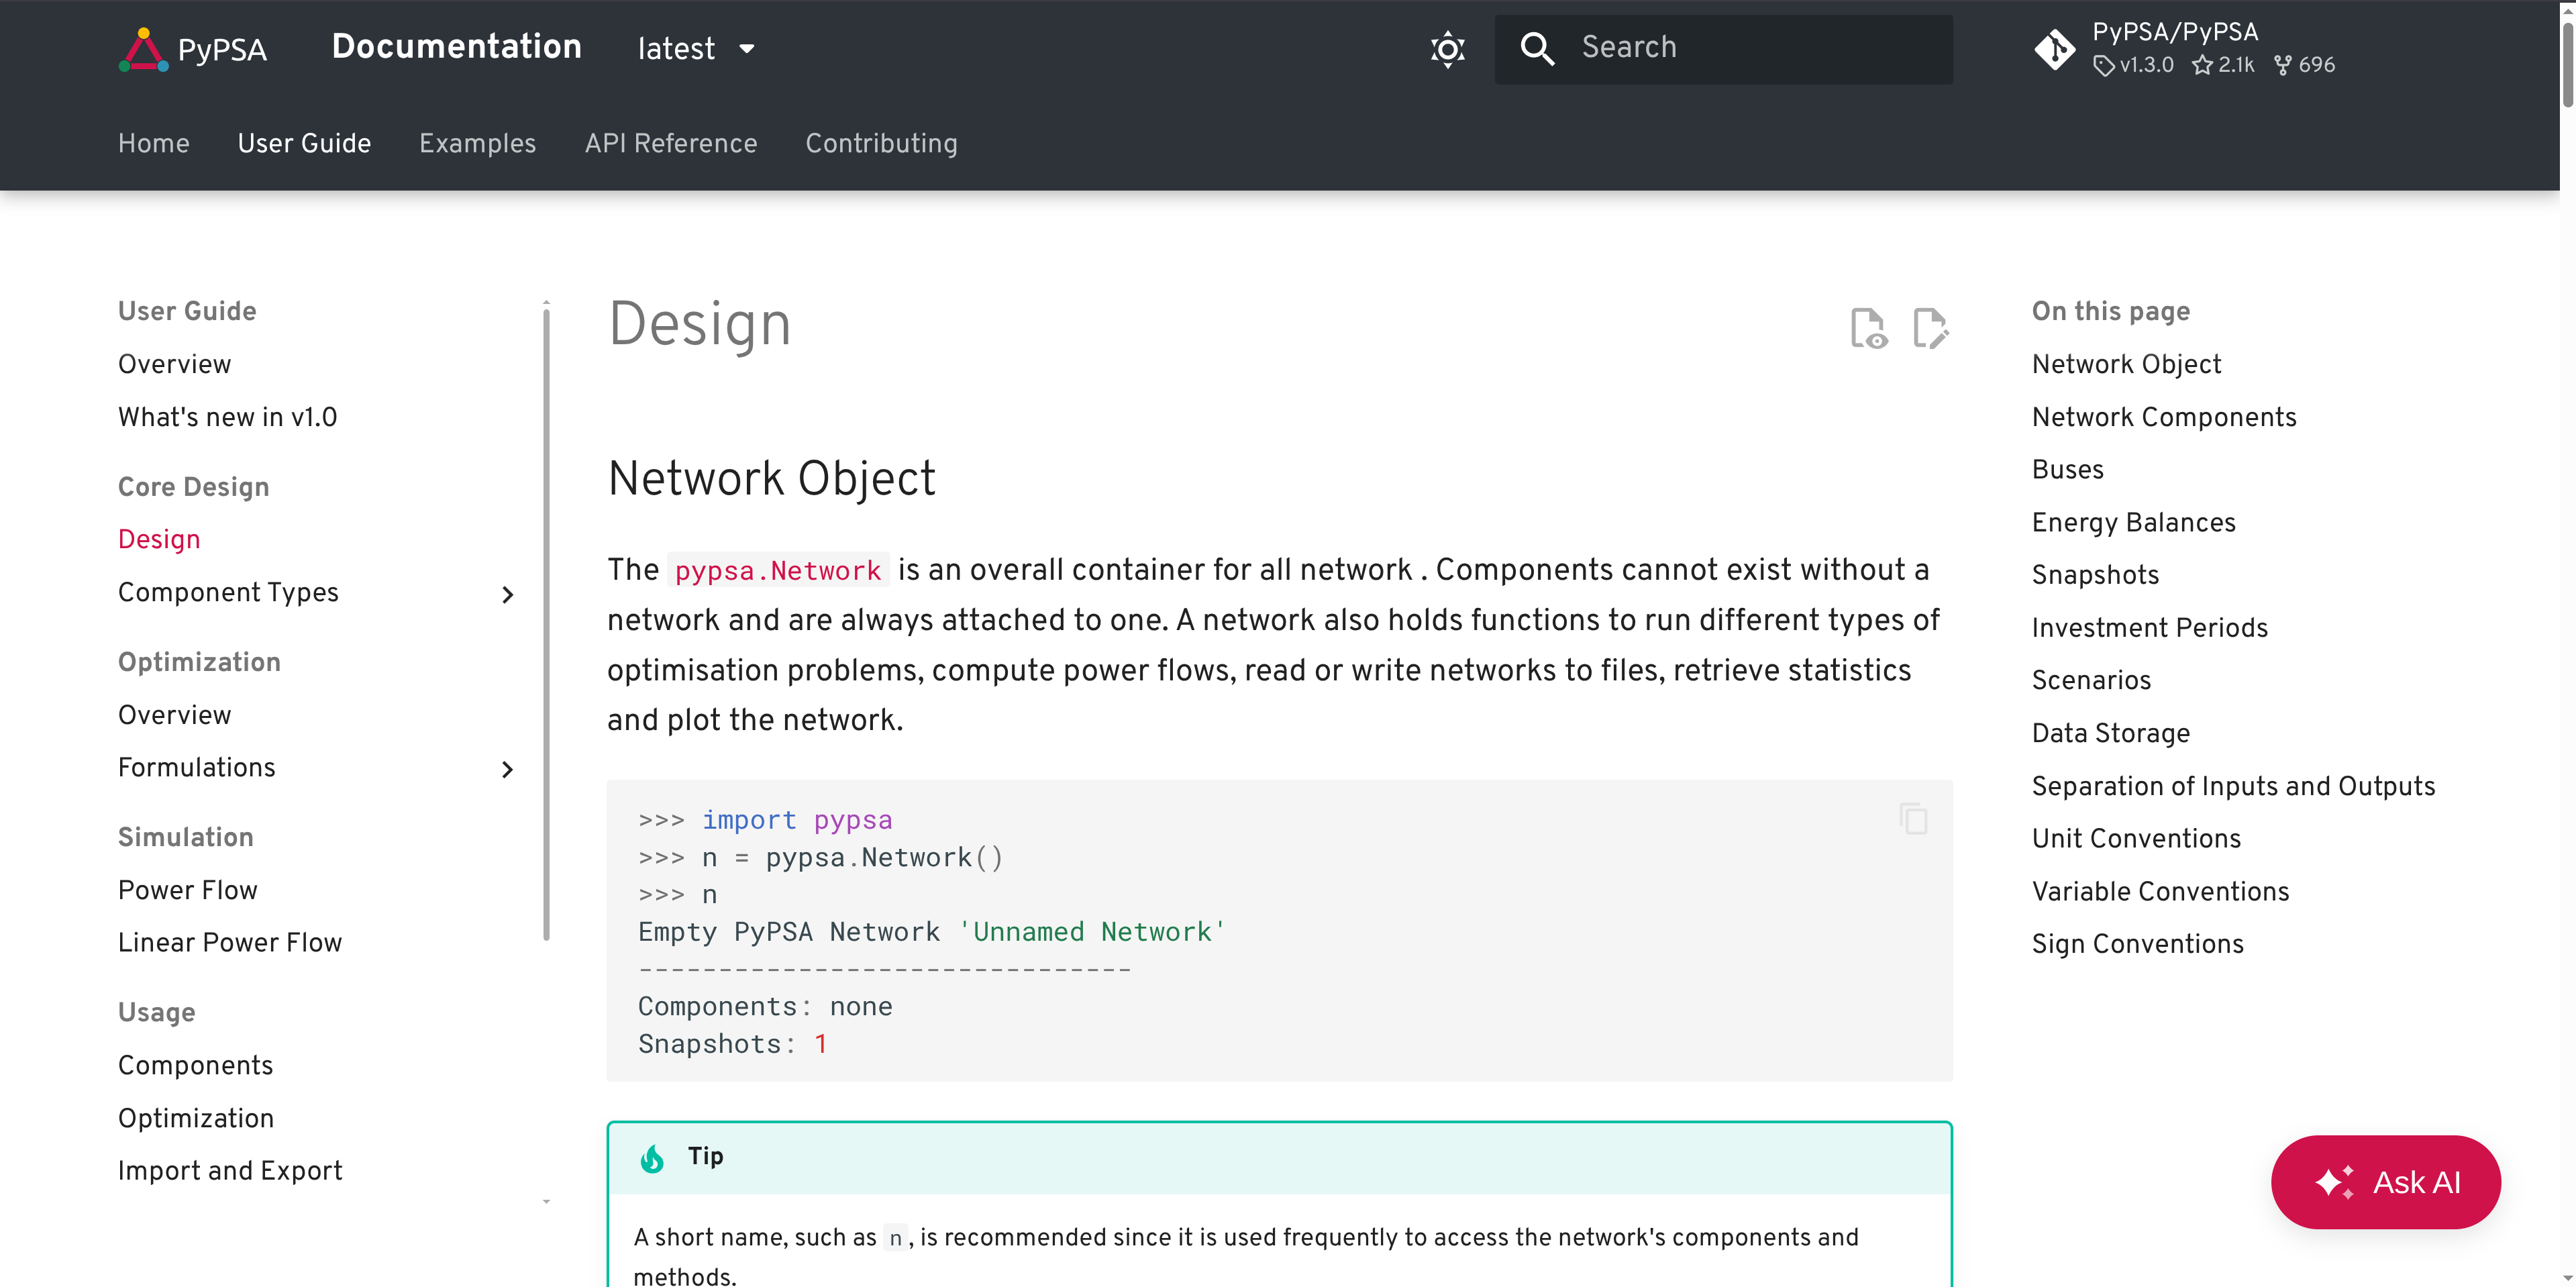
\includegraphics[width=\textwidth,keepaspectratio]{graphics/pypsa-docs.png}
\end{frame}

\section{Sustaining OS ecosystem}

\begin{frame}{}
	\begin{columns}[T,onlytextwidth]
		\begin{column}{0.58\textwidth}
			\setlength{\leftskip}{0.4cm}
			
\includegraphics[width=0.62\linewidth]{graphics/pypsa-labs.png}

			\vspace{0.25cm}
			\textbf{Sustaining open-source energy system  \\ modelling with PyPSA}

			\small
			\begin{itemize}
				\item \text{Development \& maintenance}
				\item \text{Support subscriptions}
				\item \text{Training workshops}
				\item \text{Modelling studies}
			\end{itemize}
		\end{column}
		\begin{column}{0.40\textwidth}
			\raggedright
			\vspace{0.3cm}
			\begin{minipage}{3.6cm}
				\centering
				\qrcode[height=3.6cm]{https://pypsalabs.org}\\[0.3cm]
				\normalsize\href{https://pypsalabs.org}{pypsalabs.org}
			\end{minipage}
		\end{column}
	\end{columns}

\end{frame}

\begin{frame}{The Power of Many: Open Source for Critical Infrastructure}

	\textbf{Dr. Michael Lindner}\\
	\textbf{Dr. Iegor Riepin} (iegor.riepin@tu-berlin.de)\\
	\vspace{1cm}
	\alert{PyPSA ecosystem}: \url{https://pypsa.org/} \\
	\alert{About RESILIENT project}: \url{https://resilient-project.github.io/} \\

\end{frame}

\section{Annex}

\begin{frame}{}
	\hspace*{-0.5cm}\hspace*{-0.5cm}\includegraphics[width=15cm]{graphics/5_osm.png}
\end{frame}

\begin{frame}{The Berlin blackout and the open data question}

	\begin{columns}[T,onlytextwidth]
		\begin{column}{0.22\textwidth}
			\footnotesize
			The January 2026 blackout in parts of Berlin raised attention to open infrastructure data.

			\vspace{0.4cm}
			Tools like \alert{OpenInfraMap} allow anyone to explore the topology of the electricity grid, gas pipelines, etc. at street level.

			\vspace{0.4cm}
			\href{https://openinframap.org/\#13.86/52.42948/13.30546/A,B,L,P}{openinframap.org}
		\end{column}
		\begin{column}{0.76\textwidth}
			\includegraphics[width=\linewidth]{graphics/openinframap-berlin.png}
		\end{column}
	\end{columns}

	\source{\href{https://openinframap.org/}{OpenInfraMap} · Map data \textcopyright{} \href{https://www.openstreetmap.org/copyright}{OpenStreetMap contributors} (ODbL)}

\end{frame}

\begin{frame}{Security by obscurity is a dangerous fallacy}

	\begin{columns}[T,onlytextwidth]
		\begin{column}{0.38\textwidth}
			\footnotesize
			\alert{The assumption}: restrict access to infrastructure data so adversaries can't use it. If they don't know where the lines run, they can't attack them.

			\vspace{0.3cm}
			\alert{The reality}: anyone who looks can find it
			\begin{itemize}
				\item commercial satellite imagery at \textbf{50\,cm resolution}
				\item drone imagery and street-level photos
				\item commercial geospatial datasets
				\item public grid studies and regulatory filings
				\item web archives and cached maps
			\end{itemize}

		\end{column}
		\begin{column}{0.60\textwidth}
			\vspace{0.8cm}
			\includegraphics[width=\linewidth]{graphics/substation-aerial.jpg}
		\end{column}
	\end{columns}

	\source{Aerial photo: Enniger Substation 380\,kV, \href{https://commons.wikimedia.org/wiki/File:Enniger_Substation_(380_kV_to_110_kV),_aerial_view.jpg}{Wikimedia Commons} (CC BY-SA)}

\end{frame}

\end{document}
